\documentclass{report}
\setlength{\parskip}{\baselineskip}%
\usepackage{amsmath}
\usepackage{amsfonts,stmaryrd,amssymb} % Math packages

\usepackage{enumerate} % Custom item numbers for enumerations
\usepackage{fontawesome}
\usepackage{setspace}
\usepackage{hyperref}
\usepackage{enumitem}
\usepackage{multicol}
\usepackage{xhfill}
\usepackage[p,osf]{cochineal}
\usepackage[scale=.95,type1]{cabin}
\usepackage[cochineal,bigdelims,cmintegrals,vvarbb]{newtxmath}
\usepackage[zerostyle=c,scaled=.94]{newtxtt}
\usepackage[cal=boondoxo]{mathalfa}
\usepackage[export]{adjustbox}
\usepackage{vwcol}  
\usepackage{fancyhdr}
\DeclareSymbolFont{yhlargesymbols}{OMX}{yhex}{m}{n}
\DeclareMathAccent{\wideparen}{\mathord}{yhlargesymbols}{"F3}

\hypersetup{
	colorlinks=false,
	linkcolor=black,
	filecolor=black,      
	urlcolor=black,
	pdftitle={Overleaf Example},
	pdfpagemode=FullScreen,
	urlbordercolor=white,
}

\urlstyle{same}


	
\newenvironment{cequation}{
	\makeatletter
	\setbool{@fleqn}{false}
	\makeatother
	\begin{equation*}
		}{\end{equation*}}
		
\newcommand{\sol}{\noindent\textbf{Solution:} }
%----------------------------------------------------------------------------------------

\newcommand{\exercise}[1]{%
	\subsection*{\faPencil\ \ Exercise #1\hspace{0.5em}\xrfill[0.175\baselineskip]{1pt}}
}

\newcommand{\practice}[1]{%
	\subsection*{\faFlag\ \ Practice #1\hspace{0.5em}\xrfill[0.175\baselineskip]{1pt}}
}

\newcommand{\revision}[1]{%
	\section*{\faGears\ \ Revision Exercise #1\hspace{0.5em}\xrfill[0.175\baselineskip]{1pt}}
}

\usepackage[ruled]{algorithm2e} % Algorithms

\usepackage[framemethod=tikz]{mdframed} % Allows defining custom boxed/framed environments

\usepackage{listings} % File listings, with syntax highlighting
\lstset{
	basicstyle=\ttfamily, % Typeset listings in monospace font
}

%----------------------------------------------------------------------------------------
%	DOCUMENT MARGINS
%----------------------------------------------------------------------------------------

\usepackage{geometry} % Required for adjusting page dimensions and margins

\geometry{
	paper=a4paper, % Paper size, change to letterpaper for US letter size
	top=2.5cm, % Top margin
	bottom=3cm, % Bottom margin
	left=2.5cm, % Left margin
	right=2.5cm, % Right margin
	headheight=14pt, % Header height
	footskip=1.5cm, % Space from the bottom margin to the baseline of the footer
	headsep=1.2cm, % Space from the top margin to the baseline of the header
	%showframe, % Uncomment to show how the type block is set on the page
}

%----------------------------------------------------------------------------------------
%	FONTS
%----------------------------------------------------------------------------------------

\usepackage[utf8]{inputenc} % Required for inputting international characters
\usepackage[T1]{fontenc} % Output font encoding for international characters

%----------------------------------------------------------------------------------------
%	COMMAND LINE ENVIRONMENT
%----------------------------------------------------------------------------------------

% Usage:
% \begin{commandline}
%	\begin{verbatim}
%		$ ls
%		
%		Applications	Desktop	...
%	\end{verbatim}
% \end{commandline}

\mdfdefinestyle{commandline}{
	leftmargin=10pt,
	rightmargin=10pt,
	innerleftmargin=15pt,
	middlelinecolor=black!50!white,
	middlelinewidth=2pt,
	frametitlerule=false,
	backgroundcolor=black!5!white,
	frametitle={Command Line},
	frametitlefont={\normalfont\sffamily\color{white}\hspace{-1em}},
	frametitlebackgroundcolor=black!50!white,
	nobreak,
}

% Define a custom environment for command-line snapshots
\newenvironment{commandline}{
	\medskip
	\begin{mdframed}[style=commandline]
		}{
	\end{mdframed}
	\medskip
}

%----------------------------------------------------------------------------------------
%	FILE CONTENTS ENVIRONMENT
%----------------------------------------------------------------------------------------

% Usage:
% \begin{file}[optional filename, defaults to "File"]
%	File contents, for example, with a listings environment
% \end{file}

\mdfdefinestyle{file}{
	innertopmargin=1.6\baselineskip,
	innerbottommargin=0.8\baselineskip,
	topline=false, bottomline=false,
	leftline=false, rightline=false,
	leftmargin=2cm,
	rightmargin=2cm,
	singleextra={%
		\draw[fill=black!10!white](P)++(0,-1.2em)rectangle(P-|O);
		\node[anchor=north west]
		at(P-|O){\ttfamily\mdfilename};
		%
		\def\l{3em}
		\draw(O-|P)++(-\l,0)--++(\l,\l)--(P)--(P-|O)--(O)--cycle;
		\draw(O-|P)++(-\l,0)--++(0,\l)--++(\l,0);
	},
	nobreak,
}

% Define a custom environment for file contents
\newenvironment{file}[1][File]{ % Set the default filename to "File"
	\medskip
	\newcommand{\mdfilename}{#1}
	\begin{mdframed}[style=file]
		}{
	\end{mdframed}
	\medskip
}

%----------------------------------------------------------------------------------------
%	NUMBERED QUESTIONS ENVIRONMENT
%----------------------------------------------------------------------------------------

% Usage:
% \begin{question}[optional title]
%	Question contents
% \end{question}

\mdfdefinestyle{question}{
	innertopmargin=1.2\baselineskip,
	innerbottommargin=0.8\baselineskip,
	roundcorner=5pt,
	nobreak,
	singleextra={%
		\draw(P-|O)node[xshift=1em,anchor=west,fill=white,draw,rounded corners=3pt]{%
			\faCaretRight\ \textbf{Example \theQuestion\questionTitle}};
	},
}

\newcounter{Question} % Stores the current question number that gets iterated with each new question

% Define a custom environment for numbered questions
\newenvironment{question}[1][\unskip]{
	\bigskip
	\stepcounter{Question}
	\newcommand{\questionTitle}{~#1}
	\begin{mdframed}[style=question]
		}{
	\end{mdframed}
	\medskip
}

%----------------------------------------------------------------------------------------
%	SOLUTIONS ENVIRONMENT
%----------------------------------------------------------------------------------------

% Usage:
% \begin{solution}
%	Solution contents
% \end{solution}

\mdfdefinestyle{solution}{
	innertopmargin=1.2\baselineskip,
	innerbottommargin=0.8\baselineskip,
	roundcorner=5pt,
	nobreak,
	singleextra={%
		\draw(P-|O)node[xshift=1em,anchor=west,fill=white,draw,rounded corners=5pt]{解};
	},
}

% Define a custom environment for solutions
\newenvironment{solution}{
	\begin{mdframed}[style=solution]
		}{
	\end{mdframed}
}

%----------------------------------------------------------------------------------------
%	WARNING TEXT ENVIRONMENT
%----------------------------------------------------------------------------------------

% Usage:
% \begin{warn}[optional title, defaults to "Warning:"]
%	Contents
% \end{warn}

\mdfdefinestyle{warning}{
	topline=false, bottomline=false,
	leftline=false, rightline=false,
	nobreak,
	singleextra={%
		\draw(P-|O)++(-0.5em,0)node(tmp1){};
		\draw(P-|O)++(0.5em,0)node(tmp2){};
		\fill[black,rotate around={45:(P-|O)}](tmp1)rectangle(tmp2);
		\node at(P-|O){\color{white}\scriptsize\bf !};
		\draw[very thick](P-|O)++(0,-1em)--(O);%--(O-|P);
	}
}

% Define a custom environment for warning text
\newenvironment{warn}[1][Warning:]{ % Set the default warning to "Warning:"
	\medskip
	\begin{mdframed}[style=warning]
		\noindent{\textbf{#1}}
		}{
	\end{mdframed}
	\vspace{-0.5cm}
}

%----------------------------------------------------------------------------------------
%	INFORMATION ENVIRONMENT
%----------------------------------------------------------------------------------------

% Usage:
% \begin{info}[optional title, defaults to "Info:"]
% 	contents
% 	\end{info}

\mdfdefinestyle{info}{%
	topline=false, bottomline=false,
	leftline=false, rightline=false,
	nobreak,
	singleextra={%
		\fill[black](P-|O)circle[radius=0.6em];
		\node at(P-|O){\color{white}\scriptsize\bf \faInfo};
		\draw[very thick](P-|O)++(0,-0.8em)--(O);%--(O-|P);
	}
}

% Define a custom environment for information
\newenvironment{info}[1][Info:]{ % Set the default title to "Info:"
	\medskip
	\begin{mdframed}[style=info]
		\noindent{\textbf{#1}}
		}{
	\end{mdframed}
	\vspace{-0.5cm}
	
}

\mdfdefinestyle{explore}{%
	topline=false, bottomline=false,
	leftline=false, rightline=false,
	nobreak,
	singleextra={%
		\fill[black](P-|O)circle[radius=0.6em];
		\node at(P-|O){\color{white}\scriptsize\bf \faFlask};
		\draw[very thick](P-|O)++(0,-0.8em)--(O);%--(O-|P);
	}
}

% Define a custom environment for warning text
\newenvironment{explore}[1][Exploration Activity:]{ % Set the default warning to "Warning:"
	\medskip
	\begin{mdframed}[style=explore]
		\noindent{\large\textbf{#1}}
		}{
	\end{mdframed}
	\vspace{-0.5cm}
}

\mdfdefinestyle{think}{%
	topline=false, bottomline=false,
	leftline=false, rightline=false,
	nobreak,
	singleextra={%
		\fill[black](P-|O)circle[radius=0.6em];
		\node at(P-|O){\color{white}\scriptsize\bf \faQuestion};
		\draw[very thick](P-|O)++(0,-0.8em)--(O);%--(O-|P);
	}
}

% Define a custom environment for warning text
\newenvironment{think}[1][Think about It:]{ % Set the default warning to "Warning:"
	\medskip
	\begin{mdframed}[style=think]
		\noindent{\large\textbf{#1}}
		}{
	\end{mdframed}
	\vspace{-0.5cm}
}



\usepackage{setspace}
\usepackage{hyperref}
\usepackage{enumitem}
\usepackage{multicol}
\usepackage{xhfill}
\usepackage[p,osf]{cochineal}
\usepackage[scale=.95,type1]{cabin}
\usepackage[cochineal,bigdelims,cmintegrals,vvarbb]{newtxmath}
\usepackage[zerostyle=c,scaled=.94]{newtxtt}
\usepackage[cal=boondoxo]{mathalfa}
\usepackage[export]{adjustbox}
\usepackage{vwcol}  
\DeclareSymbolFont{yhlargesymbols}{OMX}{yhex}{m}{n}
\DeclareMathAccent{\wideparen}{\mathord}{yhlargesymbols}{"F3}

\hypersetup{
    colorlinks=false,
    linkcolor=black,
    filecolor=black,      
    urlcolor=black,
    pdftitle={Overleaf Example},
    pdfpagemode=FullScreen,
    urlbordercolor=white,
    }

    \urlstyle{same}

\newenvironment{cequation}{
    \makeatletter
    \setbool{@fleqn}{false}
    \makeatother
    \begin{equation*}
        }{\end{equation*}}

\newcommand{\sol}{\noindent\textbf{Solution:} }
%----------------------------------------------------------------------------------------

\newcommand{\exercise}[1]{%
    \subsection*{\faPencil\ \ Exercise #1\hspace{0.5em}\xrfill[0.175\baselineskip]{1pt}}
}

\newcommand{\practice}[1]{%
    \subsection*{\faFlag\ \ Practice #1\hspace{0.5em}\xrfill[0.175\baselineskip]{1pt}}
}

\begin{document}
\onehalfspacing
\setcounter{chapter}{7}

\chapter{Degree and Radian}

\section{Concept and Measurement of Arbitrary Angle}

\subsection*{Arbitrary Angle}

Back in junior high, we learned that the angle is the geometric object formed by rays from the same endpoint. As shown in the figure below, whether it is from ray $OA$ to ray $OB$, or from ray $OA$ to ray $OC$, the angle can be measured as $30^\circ$.

\begin{center}
    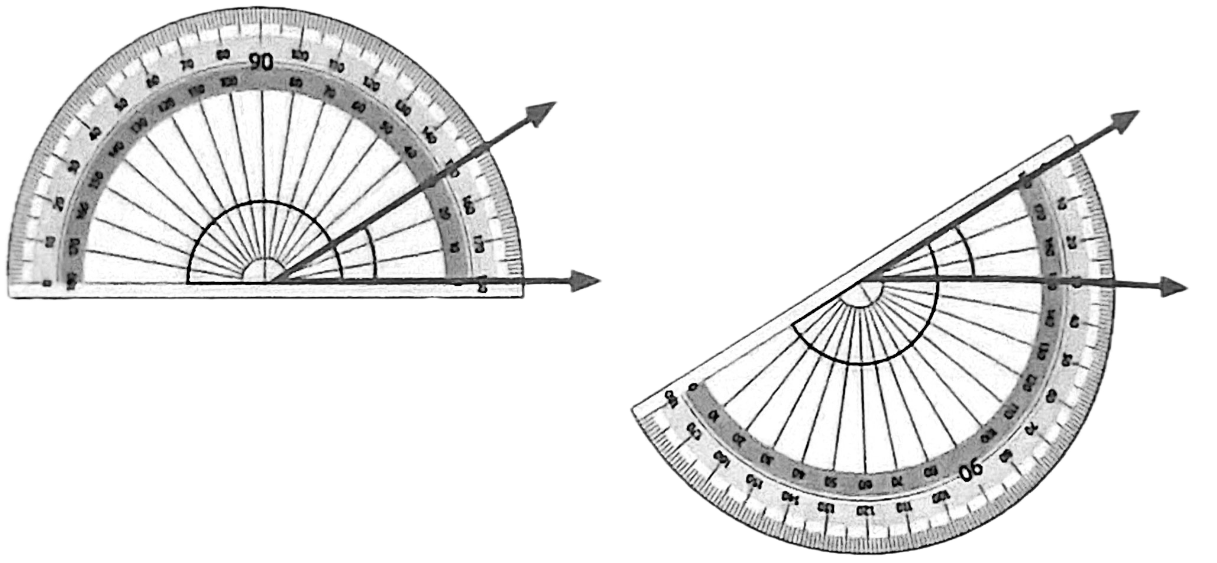
\includegraphics[scale=0.21]{assets/8-1.png}
\end{center}
\vspace{-1em}

In fact, angle can be seen as a rotation of a ray about its endpoint in a plane. As shown in the figure below, the endpoint $O$ of the ray is known as the \textbf{vertex} of the angle, the initial position $OA$ of the rotation is known as the \textbf{initial side} of the angle, and the final position $OB$ of the rotation is known as the \textbf{terminal side} of the angle, while the amount of rotation is $\angle AOB$. The rotation can be either clockwise or counterclockwise, as shown in the figure below, the angle formed counterclockwise is positive, while the angle formed clockwise is negative, $\theta > 0^\circ$ in the figure below.

\begin{center}
    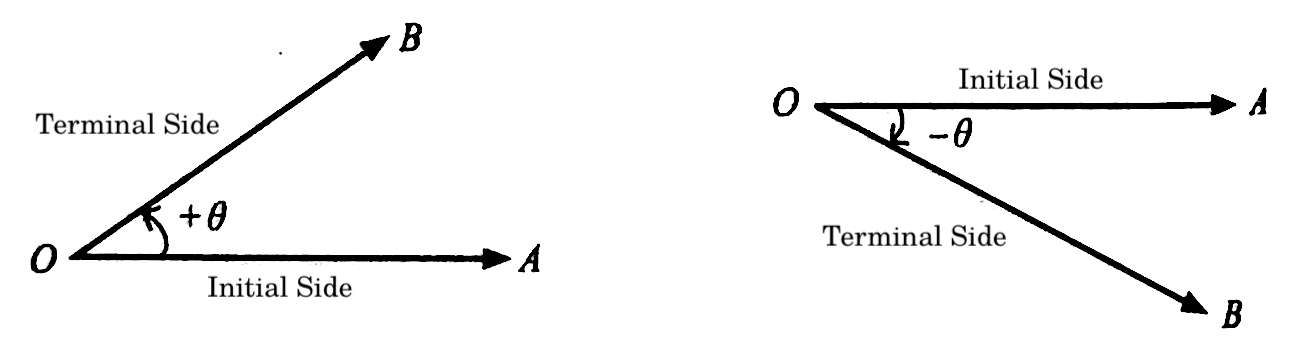
\includegraphics[scale=0.23]{assets/8-2.png}
\end{center}

\begin{explore}[Exploration Activity 1]
    
    \textbf{Aim:} To understand the definition of arbitrary angle.

    \textbf{Materials Needed:} A piece of paper, a protractor, a ruler

    \textbf{Steps:}
    \vspace{-1em}
    \begin{enumerate}
        \item Draw three parallel rays $OA$ (as shown below) on the paper. Hence, with $OA$ as the initial side of the angle, measure the following using a protractor:
        \begin{enumerate}
            \item The terminal side $OB$ of the $160^\circ$.
            \item The terminal side $OC$ of the $-45^\circ$.
            \item The terminal side $OD$ of the $450^\circ$.
        \end{enumerate}
        \item Write down clearly the respective direction and the measurement of the rotation in the three figures above.
    \end{enumerate}

    \textbf{Tool:} \underline{\url{https://www.geogebra.org/m/u7a3zxfd}}
\end{explore}

From exploration activity 1, this kind of directional rotational measurement that is not limited to $0^\circ$ to $360^\circ$ is known as the \textbf{arbitrary angle}. If the initial side doesn't rotate at all, the angle formed is called a \textbf{zero angle}.

\subsection*{Degree and Radian}

Back in junior high, the angle unit that we learned is formed by dividing a circle into $360$ equal parts, and the corresponding central angle of each part is known as 1 degree, denoted as $1^\circ$. Dividing the arc corresponding to 1 degree angle into $60$ equal parts, the corresponding central angle of each part is known as 1 minute, denoted as $1'$. Dividing the arc corresponding to 1 minute angle into $60$ equal parts, the corresponding central angle of each part is known as 1 second, denoted as $1''$.
\begin{align*}
    \therefore 1 \text{ full angle} & = 360^\circ\\
    1^\circ & = 60'\\
    1' & = 60''
\end{align*}
This form of base 60 measurement of angles is known as the \textbf{degree measure}.

\begin{explore}[Exploration Activity 2]

    \begin{enumerate}[label=\textbf{Aim:} ,leftmargin=4.5em]
        \item To inspect the relationship between arc length and radius, and to understand teh definition of radian measure.
    \end{enumerate}
    \vspace{-2em}
    \begin{enumerate}[label=\textbf{Materials Needed:} ,leftmargin=2em, align=left]
        \item A compass, a protractor, a string of length 10 cm, a scrap paper.
    \end{enumerate}
    \vspace{-1em}

    \textbf{Steps:}
    \vspace{-1em}
    \begin{enumerate}
        \item Form a group of 2 to 4 people, each group member is required to draw a circle with different radii. (Choose any arbitrary radius like 2cm, 3cm, 4cm, $\cdots$)
        
        \item Each person uses a line to measure the arc $AB$ with the same length as the radius on his own arc, then marks it on the string, as shown in the figure below.
        
        \begin{center}
            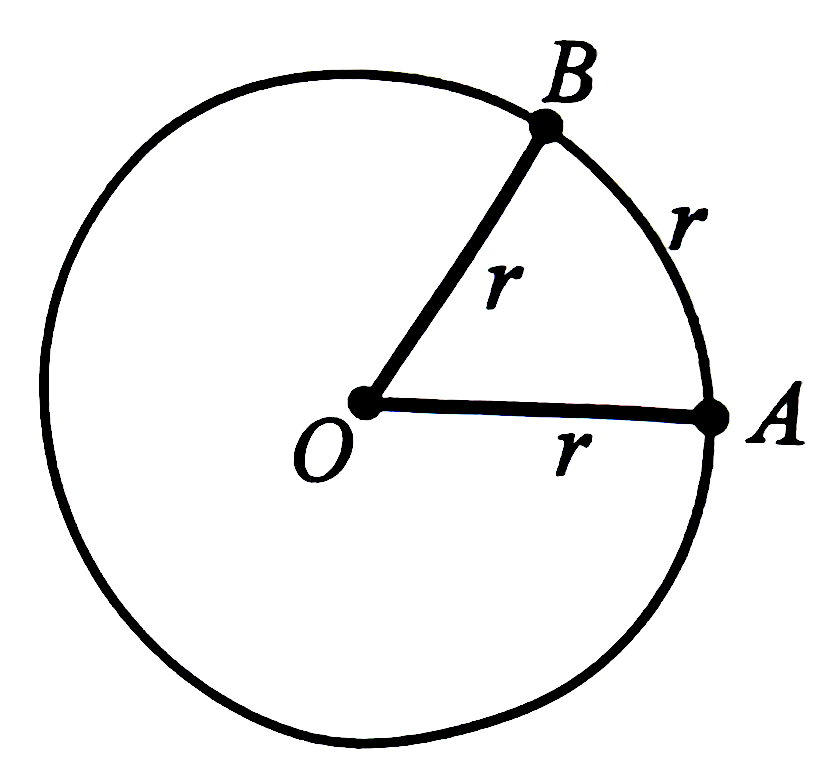
\includegraphics[scale=0.1]{assets/8-3.png}
        \end{center}
        
        \item Use a protractor to measure the corresponding central angle of the arc $AB$.
    \end{enumerate}

    \textbf{Discuss and Discover:}
    \vspace{-1em}
    \begin{enumerate}
        \item Compare the diagram drawn by each group member, are the measured central angles the same?
        \item Use a string to measure how many parts with the same length as the $AB$ of the circumference can be divided.
        \item Is it possible to derive an accurate answer for the question above using the formula of the circumference of a circle?
    \end{enumerate}
\end{explore}

From the activities above, we have led out another form of angle measurement that is commonly used in higher mathematics and other fields of science, known as the \textbf{radian measure}. We call the central angle corresponding to the arc with the same length as the radius (i.e. $\angle AOB$ in the figure above) 1 radian, denoted as $1 \text{ rad}$. From discussion 2 and discussion 3, we know that the ratio between the circumference of a circle and its radius is $2\pi$, i.e. 1 full angle $= 360^\circ = 2\pi \text{ rad}$, hence we can derive the following conversion formula between degree and radian:

\begin{info}[Conversion between Degree and Radian]
    \begin{align*}
        \pi \text{ rad} &= 180^\circ\\
        1 \text{ rad} &= \frac{180}{\pi}^\circ\\
        1^\circ &= \frac{\pi}{180} \text{ rad}
    \end{align*}
\end{info}

\begin{question}
    Convert the following angles from degree to radian:
    \vspace{-1em}
    \begin{multicols}{2}
        \begin{enumerate}[label=(\alph*)]
            \item $218.84^\circ$
            \item $48^\circ 36'$
        \end{enumerate}
    \end{multicols}
    \vspace{-1em}
    \sol{}
    \begin{enumerate}[label=(\alph*)]
        \item \begin{align*}
            218.84^\circ &= 218.84 \times \frac{\pi}{180}\\
            &= 3.8195 \text{ rad}
        \end{align*}
        \item \begin{align*}
            48^\circ 36' &= \left(48 + \frac{36}{60}\right)^{\circ}\\
            & = 48.6 \times \frac{\pi}{180}\\
            & = 0.8482 \text{ rad}
        \end{align*}
    \end{enumerate}
\end{question}

\begin{question}
    Convert 1.5 radian to degree (accurate to minute).

    \sol{}
    \begin{align*}
        1.5 \text{ rad} &= 1.5 \times \frac{180}{\pi}^\circ\\
        &= 85^\circ 57'
    \end{align*}
\end{question}

\begin{question}
    Convert $\dfrac{\pi}{45}$ radian to degree.

    \sol{}
    \begin{align*}
        \frac{\pi}{45} \text{ rad} &= \frac{\pi}{45} \times \frac{180}{\pi}^\circ\\
        &= 4^\circ
    \end{align*}
\end{question}

It is worth nothing that when we use the radian measure, the unit "radian" is usually omitted. We usually write $90^\circ = \dfrac{\pi}{2}$, but if we use degree measure to express the same angle, the unit "degree" cannot be omitted.

\practice{8.1}

\begin{enumerate}
    \item Complete the following table, express the angle in $pi$:
    
    \begin{tabular}{|l|c|c|c|c|c|c|c|c|c|c|}
        \hline Angle & $0^{\circ}$ & $30^{\circ}$ & $45^{\circ}$ & $60^{\circ}$ & $90^{\circ}$ & $120^{\circ}$ & $135^{\circ}$ & $150^{\circ}$ & $180^{\circ}$ & $270^{\circ}$ \\
        \hline Radian & & & & & & & & & & \\
        \hline
        \end{tabular}
        \vspace{1em}

        \item Convert the following angles from radian to degree (if the result is not an integer, round to 2 decimal places):
        \vspace{-1em}
        \begin{multicols}{2}
            \begin{enumerate}[label=(\alph*)]
                \item $0.5 \text{ rad}$
                \item $\dfrac{7\pi}{6} \text{ rad}$
            \end{enumerate}
        \end{multicols}
\end{enumerate}

\exercise{8.1}

\begin{enumerate}
    \item Using the horizontal ray $OA$ in the figure below as the initial side, sketch the position of the terminal side $OB$ of the following angles:
    \begin{center}
        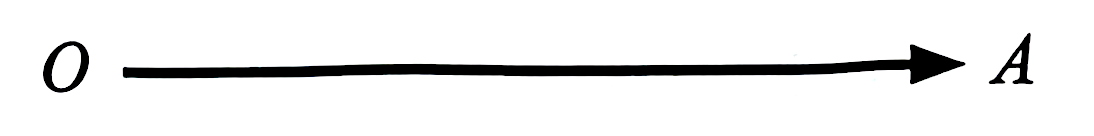
\includegraphics[scale=0.15]{assets/8-4.png}
    \end{center}
    \vspace{-1em}
    \begin{multicols}{3}
        \begin{enumerate}[label=(\alph*)]
            \item $\dfrac{5 \pi}{4}$
            \item $-\dfrac{6 \pi}{7}$
            \item $\dfrac{5 \pi}{2}$
        \end{enumerate}
    \end{multicols}
    
    \item Convert the following angles from degree to radian (accurate to 4 decimal places):
    \vspace{-1em}
    \begin{multicols}{3}
        \begin{enumerate}[label=(\alph*)]
            \item $68^\circ 93'$
            \item $139^\circ 12'$
            \item $-502^\circ 46'$
        \end{enumerate}
    \end{multicols}

    \item Convert the following angles from radian to degree (if the result is not an integer, round to minute):
    \vspace{-1em}
    \begin{multicols}{3}
        \begin{enumerate}[label=(\alph*)]
            \item $0.89 \text{ rad}$
            \item $-\dfrac{17\pi}{4} \text{ rad}$
            \item $3 \text{ rad}$
        \end{enumerate}
    \end{multicols}

    \item If the gear in the figure below rotates counterclockwise about its origin $O$, how many radians does the gear rotate through such that
    \begin{center}
        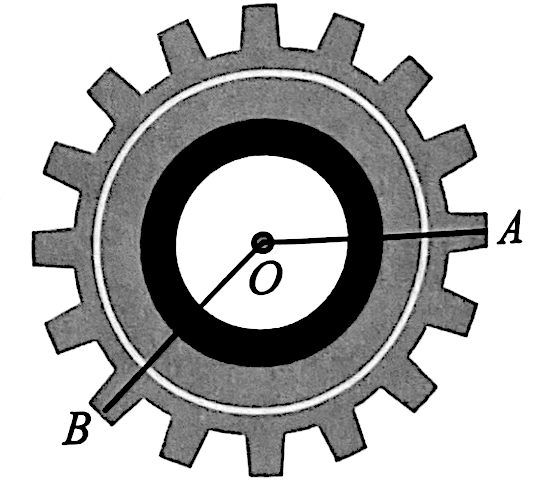
\includegraphics[scale=0.2]{assets/8-5.png}
    \end{center}
    \begin{enumerate}
        \item The line segment $OB$ reaches the position of $OA$ in the figure above for the first time?
        \item The line segment $OB$ reaches the position of $OA$ in the figure above for the second time?
    \end{enumerate}
\end{enumerate}

\newpage
\section{Arc Length and Sector Area}

\subsection*{Formula of Arc Length}

Back in junior high, we learned that in a circle with radius $r$ and central angle $\theta$,
\vspace{-1em}
\begin{enumerate}[label=(\arabic*)]
    \item if the angle is expressed in degree, the arc length $l$ is given by
    \begin{cequation}
        l = \frac{\theta}{360^\circ} \times 2\pi r\qquad(\text{where }\theta \text{ is in degree})
    \end{cequation}
    \item if the angle is expressed in radian, i.e. $360^\circ = 2\pi$, the arc length $l$ is given by
    \begin{cequation}
        l = \dfrac{\theta}{2\pi} \times 2\pi r = \theta r\qquad(\text{where }\theta \text{ is in radian})
    \end{cequation}
\end{enumerate}

From the definition of radians, we can see that if the central angle corresponding to the arc $AB$ is $\theta$ radian, then the arc length $AB$ is $\theta$ times the length of radius $r$. That is,
    \begin{info}[Formula of Arc Length]
        \begin{cequation}
            \theta = \frac{l}{r}
        \end{cequation}
        \vspace{-1em}
        \begin{cequation}
            r = \frac{l}{\theta}
        \end{cequation}
        \vspace{-1em}
    \end{info}

\begin{question}
    In a circle with radius 5 cm, find
    \vspace{-1em}
    \begin{enumerate}[label=(\alph*)]
        \item The arc length corresponding to the central angle of $1.5 \text{ rad}$.
        \item The central angle corresponding to the arc length of 17 cm.
    \end{enumerate}
    \sol{}
    \begin{enumerate}[label=(\alph*)]
        \item $\begin{aligned}[t]
            \text{The corresponding arc length} &= 1.5 \times 5\\
            &= 7.5 \text{ cm}
        \end{aligned}$
        \item Let $\theta$ be the central angle, then
        \begin{align*}
            5\theta &= 17&\\
            \theta &= 3.4
        \end{align*}
        The central angle corresponding to the arc length of 17 cm is $3.4 \text{ rad}$.
    \end{enumerate}
\end{question}

\begin{question}
    \begin{center}
        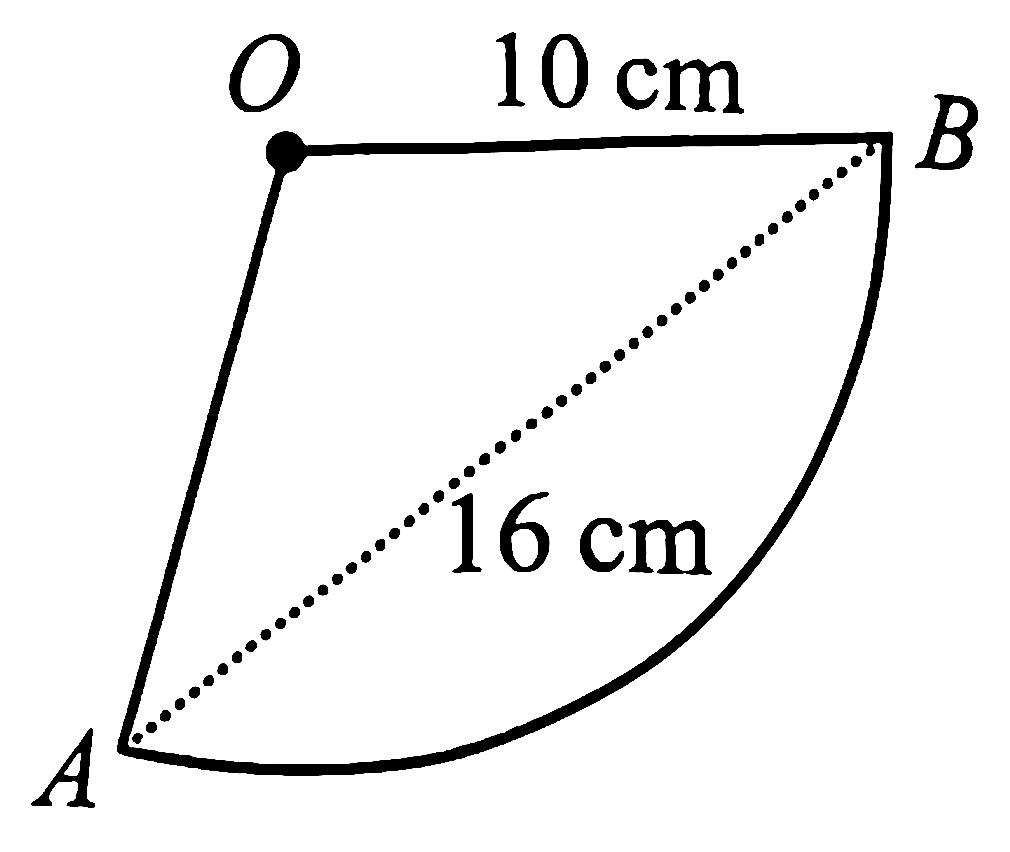
\includegraphics[scale=0.09]{assets/8-6.png}
    \end{center}
    \noindent The figure above shows a sector with center $O$ and radius of 10 cm. If the length of chord $AB$ is 16 cm, find
    \vspace{-1em}
    \begin{multicols}{2}
        \begin{enumerate}[label=(\alph*)]
            \item $\angle AOB$ (in radian);
            \item The length of arc $AB$.
        \end{enumerate}
    \end{multicols}
    \vspace{-1em}
    \sol{}
    \begin{enumerate}[label=(\alph*)]
        \item \begin{multicols}{2}
            Let $M$ be the midpoint of chord $AB$,
        
        $\therefore$ $OM \perp AB$ and $\angle MOB = \angle MOA$
        \begin{flalign*}
            \text{In }\triangle OMB,&\text{$\qquad$$\begin{aligned}[t]
                \sin \angle BOM &= \dfrac{MB}{OB} &\\
                &= \dfrac{8}{10}\\
                \angle BOM &= 0.9273
            \end{aligned}$}\\
            \text{Hence},&\text{$\qquad$$\begin{aligned}[t]
                \angle AOB &= 2 \times 0.9273\\
                &= 1.8546 \text{ rad}
            \end{aligned}$}&
        \end{flalign*}
            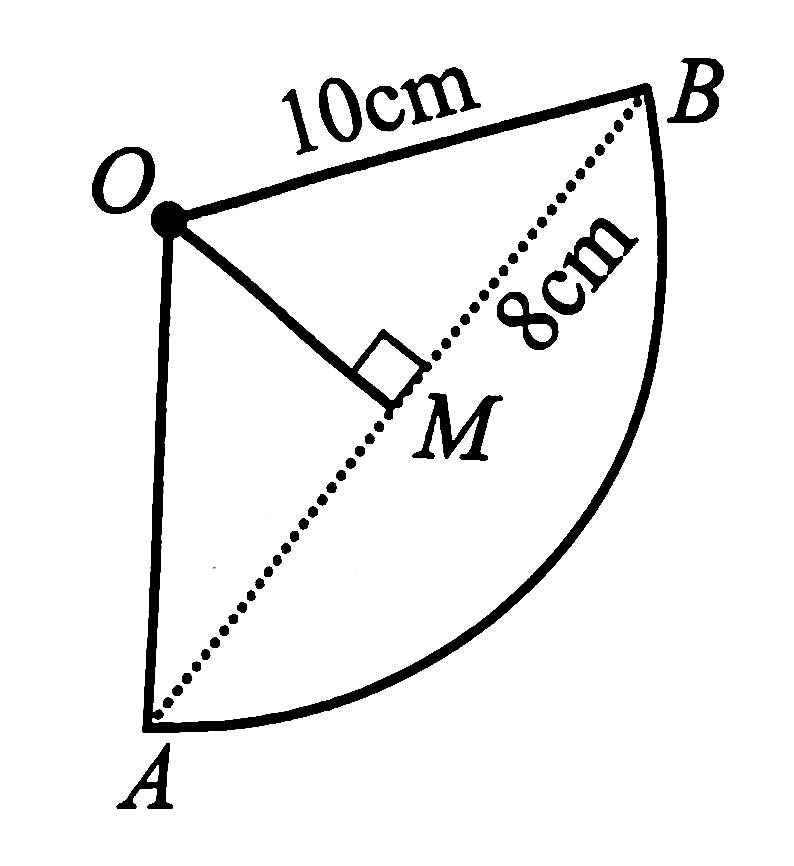
\includegraphics[scale=0.12]{assets/8-7.png}
        \end{multicols}
        \item $\begin{aligned}[t]
            \text{Arc length } AB &= 1.8546 \times 10\\
            &= 18.546 \text{ cm}
        \end{aligned}$
    \end{enumerate}
\end{question}
\begin{info}[Knowledge Review]
        
    \noindent The trigonometric functions that we learned in junior high are:
    \begin{multicols}{2}
        \vspace*{-3em}
        \begin{align*}
            \sin \theta &= \dfrac{y}{r}\\
            \cos \theta &= \dfrac{x}{r}\\
            \tan \theta &= \dfrac{y}{x}
        \end{align*}
        \columnbreak
        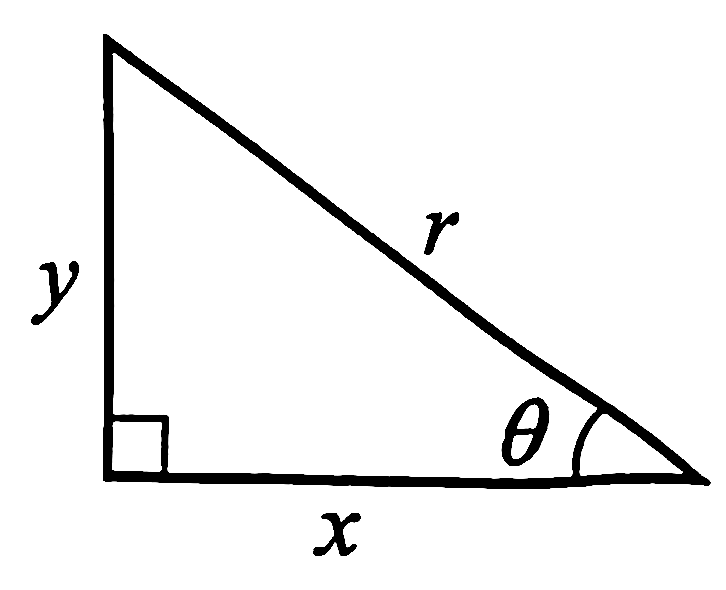
\includegraphics[scale=0.12]{assets/8-8.png}
    \end{multicols}
    \vspace{-2em}
    Adding appropriate auxiliary lines to form a right angle triangle, we can use the trigonometric functions to find the relationship between the sides and the angles of the triangle.
\end{info}
\vspace{1em}
\begin{think}
   
    \noindent Can we use degree to find the arc length $AB$?
\end{think}

\practice{8.2a}

Find the circumference of the following sectors:
\begin{multicols}{2}
    \begin{enumerate}[label=(\alph*)]
        \item 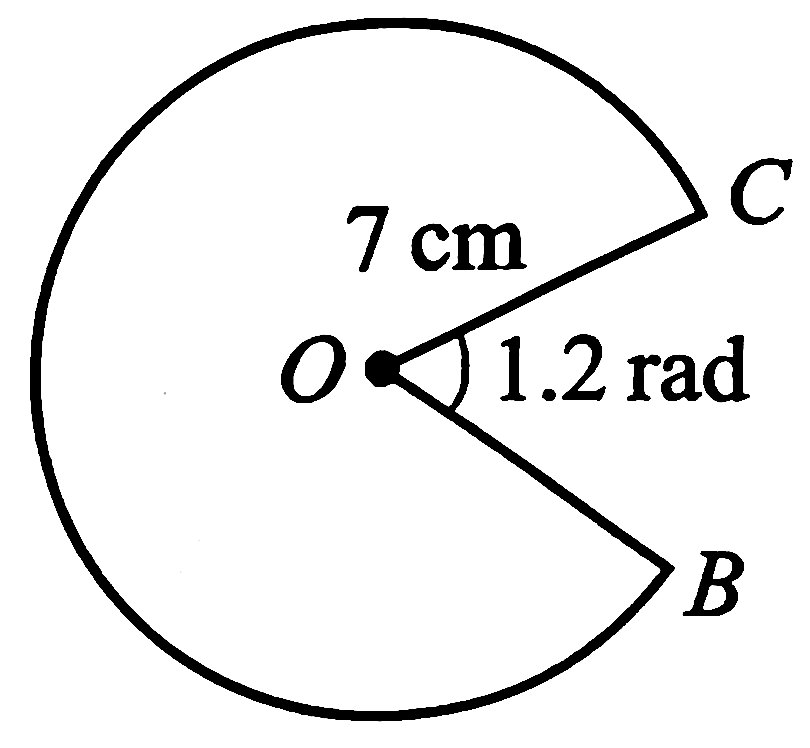
\includegraphics[scale=0.12,valign=t]{assets/8-9.png}
        \item 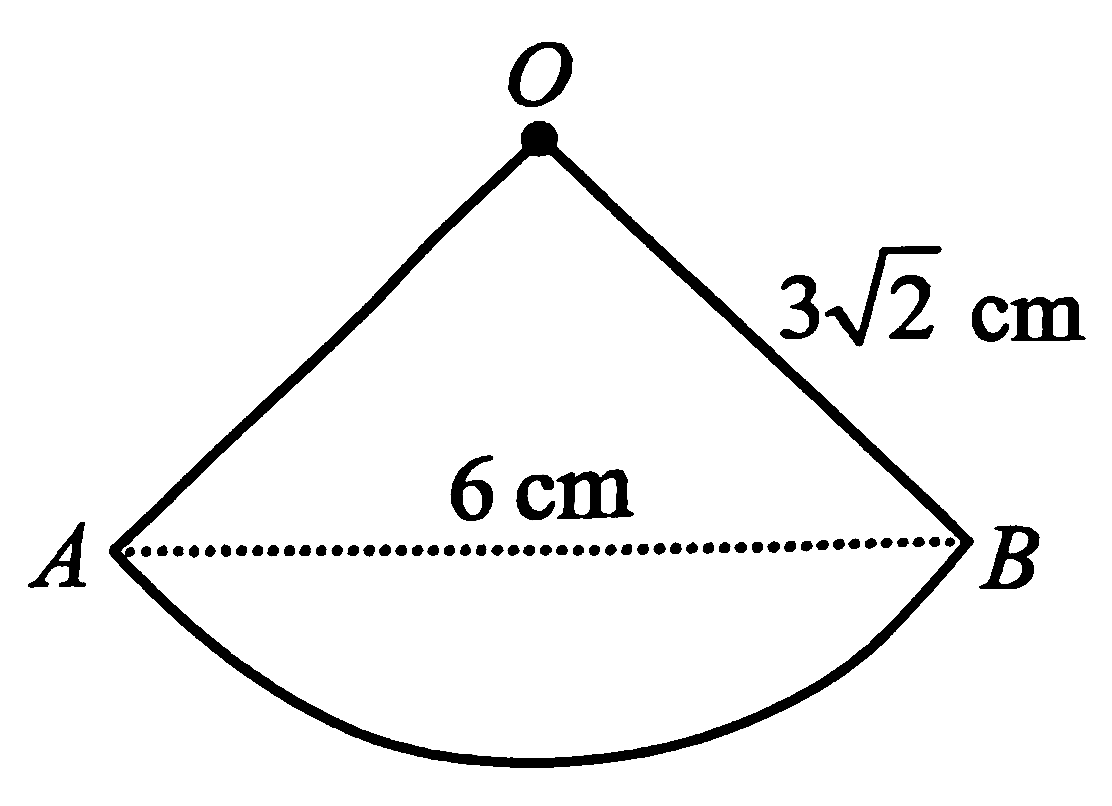
\includegraphics[scale=0.12,valign=t]{assets/8-10.png}
    \end{enumerate}
\end{multicols}

\subsection*{Formula of Sector Area}

\begin{explore}[Exploration Activity 3]
        
        \begin{enumerate}[label=\textbf{Aim:} ,leftmargin=4.4em]
            \item To strengthen the understanding of the relationship between the ratio of radian and arc length, and the ratio of radian and sector area.
        \end{enumerate}
        \vspace{-2em}
        \begin{enumerate}[label=\textbf{Tool:} ,leftmargin=2em, align=left]
            \item \url{https://www.geogebra.org/m/a4brp8yg}
        \end{enumerate}
        \vspace{-1em}
        
        \textbf{Steps:}
        \vspace{-1em}
        \begin{enumerate}
            \item Without moving point $B$, move the radius of the circle by moving the slider $L$, and inspect the changes of the following three ratios by the coloured section of the sector:
            \begin{enumerate}[label=(\arabic*)]
                \item $\angle AOB$ and $2\pi$ rad (i.e. $360^\circ$).
                \item The arc length $AB$ and the circumference of the circle.
                \item The area of sector $OAB$ and the area of the circle.
            \end{enumerate}
            \item Without changing the radius of the circle, move point $B$ to change the central angle, and inspect the changes of the same three ratios above.
        \end{enumerate}

        From the inspection above, Have you found any identical values?
\end{explore}

\newpage

Back in junior, we learned that the area of a sector is proportional to the central angle of the sector. Hence, we can derive that
\begin{cequation}
    \text{Area of sector } = \frac{\theta}{360^\circ} \times \pi r^2\qquad(\text{where }\theta \text{ is in degree})
\end{cequation}
Since $360^\circ = 2\pi$,
\begin{cequation}
    \therefore \text{Area of sector }S = \frac{\theta}{2\pi} \times \pi r^2 \qquad(\text{where }\theta \text{ is in radian})
\end{cequation}
That is,
\begin{info}[Formula of Sector Area]
    \begin{cequation}
        S = \frac{1}{2} r^2 \theta
    \end{cequation}
    \vspace{-1em}
\end{info}
Because arc length $l = r\theta$,
$\therefore$ the area formula of a sector can also be expressed as
\begin{info}[Formula of Sector Area]
    \begin{align*}
        S &= \frac{1}{2} \times \pi r \times r\\
        S &= \frac{1}{2} r l
    \end{align*}
\end{info}

\begin{question}
    There is a sector with radius 3cm and area 15 cm$^2$. Find the central and the circumference of the sector.

    \sol{}
    \vspace{-1em}
    \setlength{\columnsep}{-30em}
    \begin{multicols}{2}
        \vspace*{-2.6em}
        \begin{align*}
            S &= \dfrac{1}{2}\pi r^2\\
            15 &= \dfrac{1}{2}\pi(3)^2\\
            \theta &= \dfrac{10}{3}
        \end{align*}
        \begin{align*}
            S &= \dfrac{1}{2}lr\\
            15 &= \dfrac{1}{2}l \times 3\\
            l &= 10
        \end{align*}
    \end{multicols}
    \vspace{-4em}
    \begin{align*}
        \therefore\ \text{The central angle} &= \dfrac{10}{3} \text{ rad,}\\
        \text{The circumference} &= l + 2r\\
        &= 10 + 2 \times 3\\
        &= 16 \text{ cm}
    \end{align*}
\end{question}
\newpage
\begin{question}
    \begin{center}
        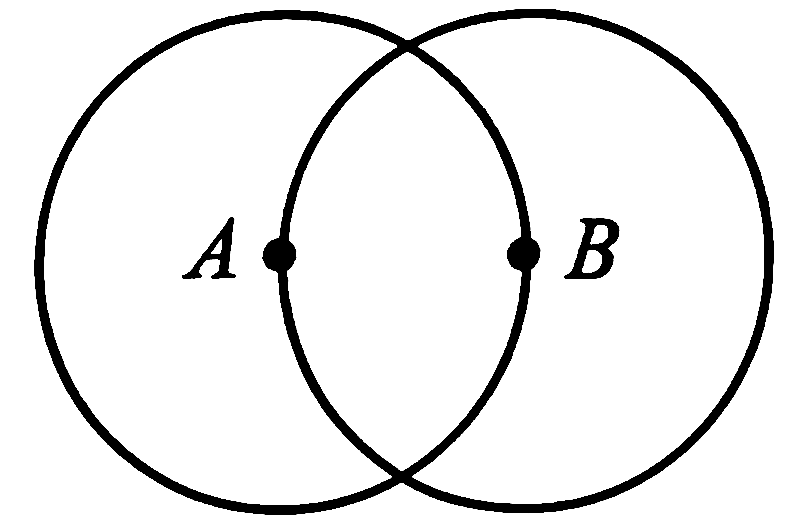
\includegraphics[scale=0.12]{assets/8-11.png}
    \end{center}
    \noindent The figure above shows two circles with the same radius $r$ and the center being $A$ and $B$ respectively. Prove that the area of the overlapping region of these two circles is $\dfrac{2}{3} \pi r^2 - \dfrac{\sqrt{3}}{2}r^2$.

    \sol{}

    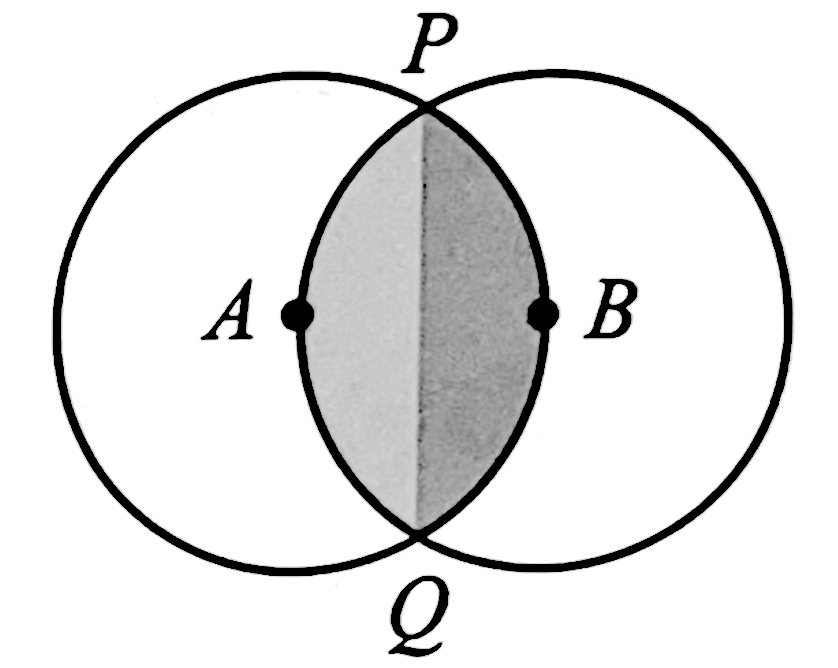
\includegraphics[scale=0.12]{assets/8-12.png}
    
    \noindent Let the two circles intersect at point $P$ and $Q$,
    
    \vspace{-1em}
    \noindent Since the two circles are of the same size, the overlapping area is formed by two identical arches.
    \begin{flalign*}
        \because &\ \triangle ABP \text{ and} \triangle ABQ \text{ are equilateral triangles,}&\\
        \therefore &\ \angle PAB = \angle BAQ = \dfrac{\pi}{3} &
    \end{flalign*}
    \vspace*{-2em}
    \begin{vwcol}[widths={0.7,0.3},rule=0pt,sep=3em]
        Let $PQ$ and $AB$ intersect at point $M$, $M$ happens to be the midpoint of line segment $PQ$ and $AB$.

        \vspace{1em}
    \noindent$\therefore AM = \dfrac{1}{2}AB = \dfrac{1}{2}r$
    \begin{flalign*}
        \text{In }\triangle AMP,\ \sin\dfrac{\pi}{3} & = \dfrac{MP}{AP}\\
        MP &= \dfrac{\sqrt{3}}{2}r&
    \end{flalign*}
    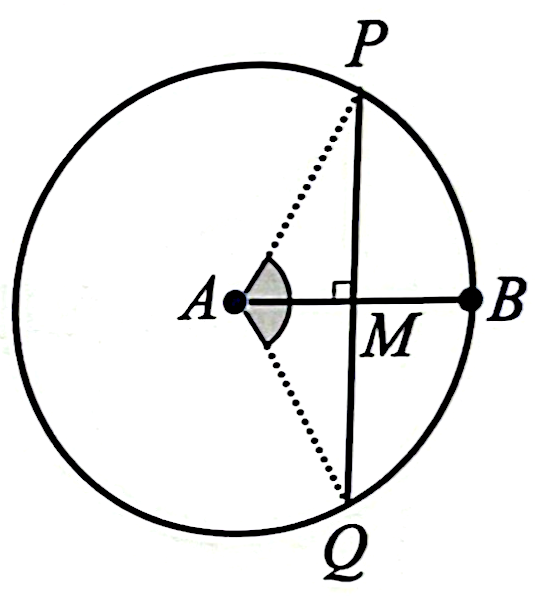
\includegraphics[scale=0.16]{assets/8-13.png}
    \end{vwcol}
    \vspace*{-2em}
    \begin{vwcol}[widths={0.2,0.8},rule=0pt,sep=3em]
        \vspace{-2.8em}
        \begin{align*}
            &\text{Area of sector } APQ&\\
            &= \dfrac{1}{2}r^2\left(\dfrac{2\pi}{3}\right) &\\
            &= \dfrac{\pi r^2}{3}
        \end{align*}
        \begin{align*}
            &\text{Area of } \triangle APQ &\\
            &= 2 \times \dfrac{1}{2}\left(\dfrac{1}{2}r\right)\left(\dfrac{\sqrt{3}}{2}r\right) &\\
            &= \dfrac{\sqrt{3}}{4}r^2
        \end{align*}
    \end{vwcol}
    \vspace{-4em}
    \begin{flalign*}
        \text{Hence, the area of the overlapping region of the two circles } &= 2 \times \left(\text{Area of sector } APQ - \text{Area of } \triangle APQ\right)&\\
        &= 2 \times \left[\dfrac{1}{3}\pi r^2 - \dfrac{\sqrt{3}}{4}r^2\right]&\\
        &= \dfrac{2}{3}\pi r^2 - \dfrac{\sqrt{3}}{2}r^2&
    \end{flalign*}
\end{question}

\newpage
\begin{question}
    \begin{vwcol}[widths={0.6,0.4},rule=0pt,sep=-10em]
        As shown in the figure to the right, both the centers of the circles with arcs $\wideparen{AB}$ and $\wideparen{CD}$ is $O$. Given that $AC = d$, $\wideparen{AB} = l'$, and $\wideparen{CD} = l$. Prove that:
        
        \vspace{1em}
        \noindent \hspace{1em}(a) $\angle AOB = \dfrac{l - l'}{d}$ radian;
        
        \noindent \hspace{1em}(b) The shaded area $= \dfrac{1}{2}(l + l')d$.
        
        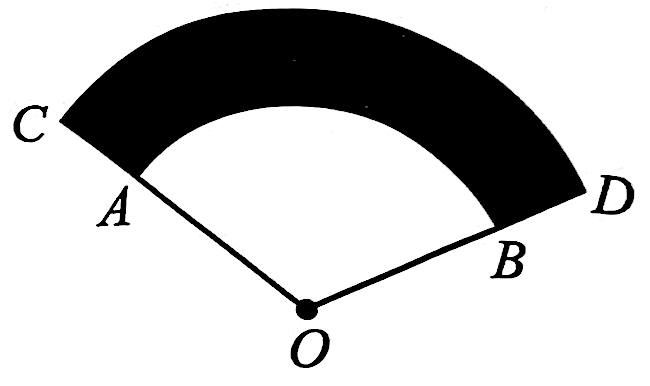
\includegraphics[scale=0.2]{assets/8-14.png}
    \end{vwcol}
        
    \sol{}
    \vspace{-1em}
    \begin{enumerate}[label=(\alph*)]
        \item Let $\begin{aligned}[t]
            \angle AOB &= \theta,\\
            l' &= (OA)\theta\\
            l &= (OC)\theta\\
            l - l' &= (OC - OA)\theta\\
            & = d\theta\\
            \theta &= \dfrac{l - l'}{d}
        \end{aligned}$
        
        \item $\begin{aligned}[t]
        \text{Area of shaded region} &= \text{Area of sector} OCD - \text{Area of sector} OAB\\
            & = \dfrac{1}{2}(OC)^2\theta - \dfrac{1}{2}(OA)^2\theta\\
            &= \dfrac{1}{2}\theta\left[(OC)^2 - (OA)^2\right]\\
            &= \dfrac{1}{2}\left[OC + OA\right]\left[OC - OA\right]\theta \qquad \because l + l' = (OC + OA)\theta\\
            & = \dfrac{1}{2}d(l + l')
        \end{aligned}$
    \end{enumerate}
\end{question}

\practice{8.2b}

Find the area of the shaded regions in the following figures:
\begin{multicols}{2}
    \begin{enumerate}[label=(\alph*)]
        \item 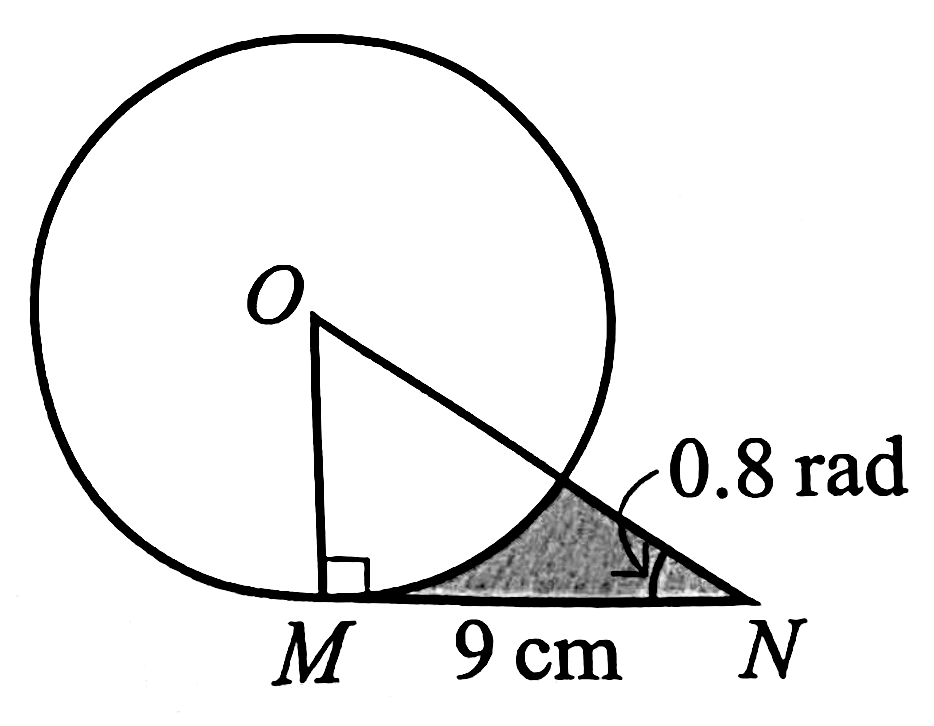
\includegraphics[scale=0.12,valign=t]{assets/8-15.png}
        \item $OAC$ is a sector, $OABC$ is a rhombus
        
        \vspace{0.5em}
        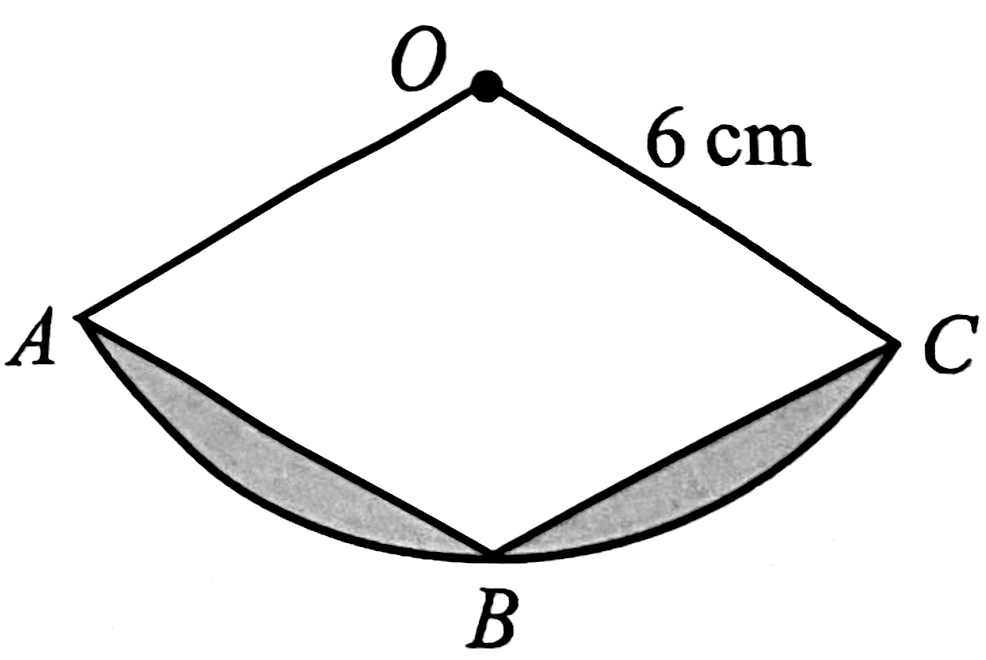
\includegraphics[scale=0.12]{assets/8-16.png}
    \end{enumerate}
\end{multicols}

\newpage

\exercise{8.2a}

\begin{enumerate}
    \item \begin{multicols}{2}
        The right figure shows a semicircle with center $O$ and diameter $8$ cm. $C$ is a point on arc $AB$. Given that $\angle CAB=0.5$ rad, find the length of arc $BC$ and the area of the shaded region.

        \begin{center}
            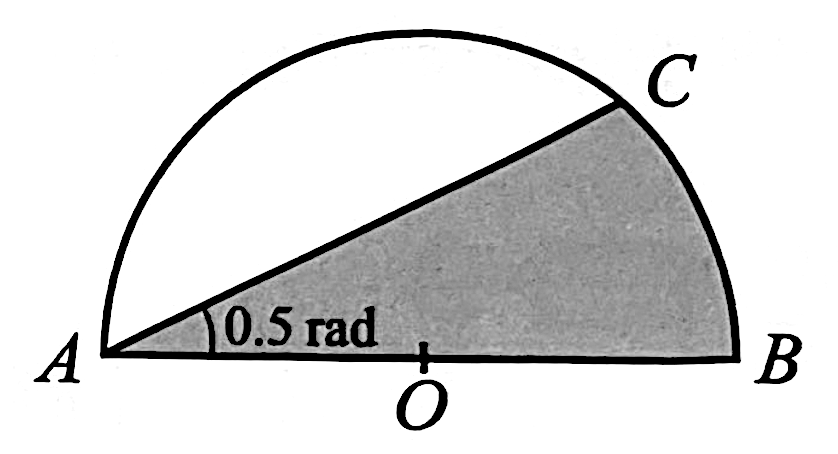
\includegraphics[scale=0.14]{assets/8-17.png}
        \end{center}
    \end{multicols}

    \item Given that the arc length of a sector is $8 \pi \mathrm{cm}$ and the area is $48 \pi \mathrm{cm}^2$, determine the radius and the central angle of the sector.

    \item \begin{multicols}{2}
        The circle in the right figure is formed by a major sector $OACB$ and a minor sector $OAB$. If the area of the major sector $OACB$ is $30 \pi \mathrm{cm}^2$, and the length of the minor arc $AB$ is $2 \pi \mathrm{cm}$, find the radius of the circle and the central angles of the two sectors.

        \begin{center}
            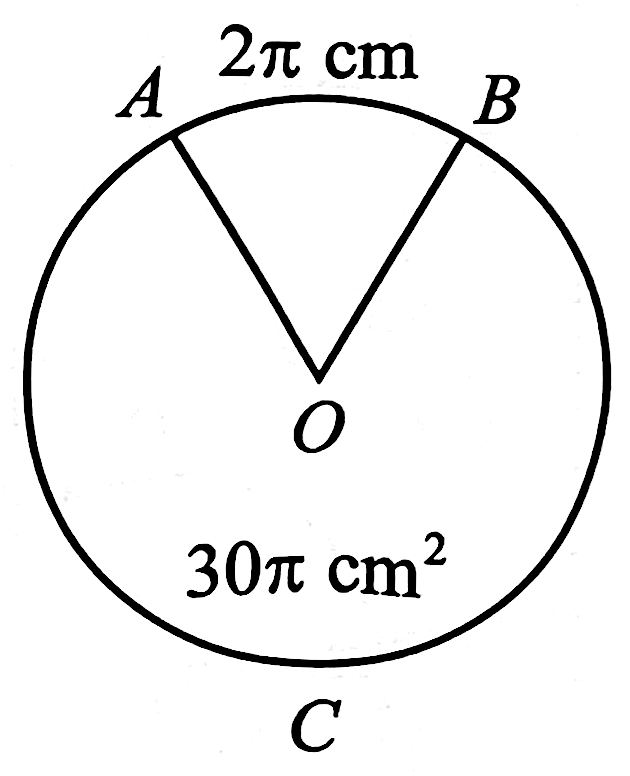
\includegraphics[scale=0.14]{assets/8-18.png}
        \end{center}
    \end{multicols}

    \item \begin{multicols}{2}
        As shown in the figure, a circle with center $C$ is tangent to the sector $OAB$ at points $P$, $Q$, and $R$. Given that $CP=4 \mathrm{~cm}$ and $\angle AOB=60^{\circ}$, without using a computer, find:
        \begin{enumerate}
            \item the length of $OA$;
            \item the area of the major sector $CPRQ$;
            \item the area of the shaded region.
        \end{enumerate}

        \begin{center}
            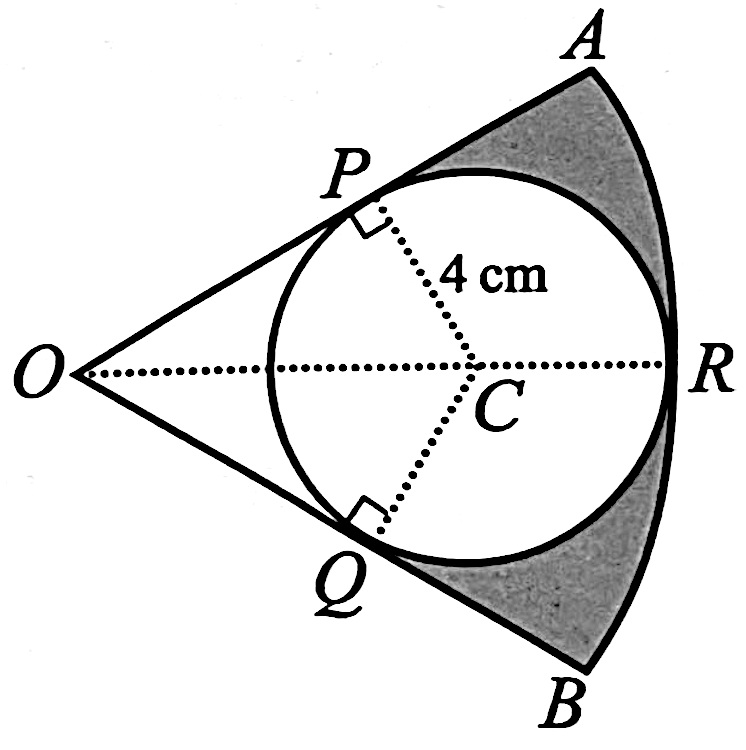
\includegraphics[scale=0.14]{assets/8-19.png}
        \end{center}
    \end{multicols}

    \item \begin{multicols}{2}
        In the right figure, $ABCD$ is a square with a side length of $a$. Four semicircles are drawn with the sides of the square as their diameters. These semicircles enclose the shaded region in the figure. Find the area of the shaded region.

        \begin{center}
            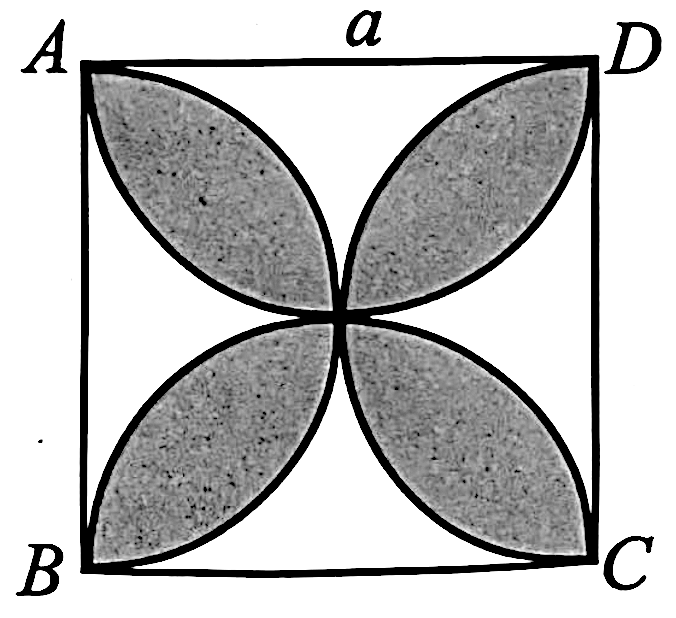
\includegraphics[scale=0.14]{assets/8-20.png}
        \end{center}
    \end{multicols}

    \item \begin{multicols}{2}
        In the right figure, $O_1$ and $O_2$ are the centers of the large and small circles respectively. The two circles are tangent to each other at point $A$, line $O_1CB$ intersects the large and small circles at points $B$ and $C$ respectively. Prove that $\wideparen{AB}=\wideparen{AC}$.

        \begin{center}
            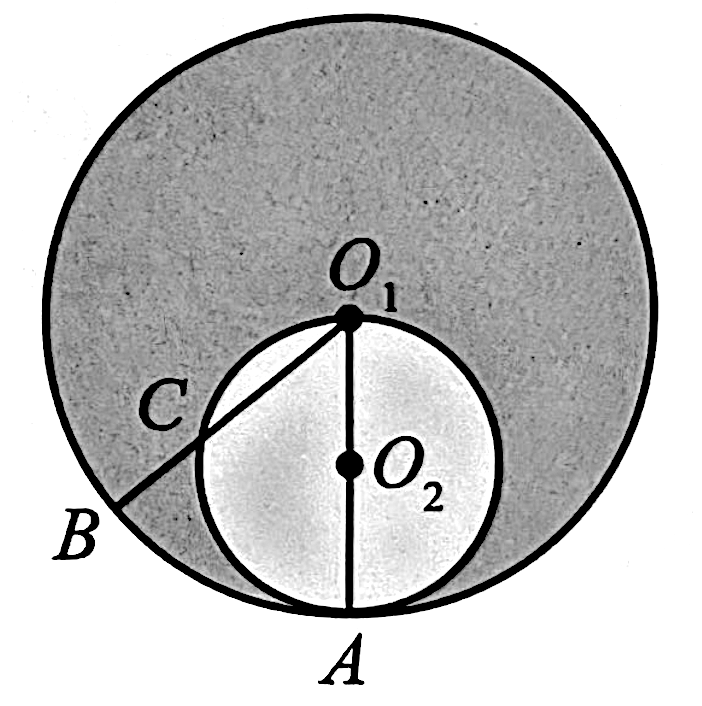
\includegraphics[scale=0.14]{assets/8-21.png}
        \end{center}
    \end{multicols}
\end{enumerate}

\newpage
\subsection*{Problems related to Arc Length and Sector}
\end{document}
